
\documentclass[letterpaper,hide notes,xcolor={table,svgnames},pdftex,10pt]{beamer}
\def\showexamples{t}

\usecolortheme{crane}
\setbeamertemplate{navigation symbols}{}

\usetheme{MyPittsburgh}
\usepackage{hyperref}
\usepackage{graphicx,xspace}
\usepackage[normalem]{ulem}
\usepackage{multicol}
\usepackage{amsmath,amssymb,amsthm,graphicx,xspace}
\newcommand\SF[1]{$\bigstar$\footnote{SF: #1}}

\usepackage[sfdefault,lf]{carlito}
\usepackage[T1]{fontenc}
\usepackage[scaled]{beramono}
\usepackage{tikzpagenodes}
\newcommand{\Rplus}{\protect\hspace{-.1em}\protect\raisebox{.35ex}{\small{\small\textbf{+}}}}
\newcommand{\Cpp}{\mbox{C\Rplus\Rplus}\xspace}

\newcounter{tmpnumSlide}
\newcounter{tmpnumNote}

\newcommand\mnote[1]{%
	\addtocounter{tmpnumSlide}{1}
	\ifdefined\showcues {~\tiny\fbox{\arabic{tmpnumSlide}}}\fi
	\note{\setlength{\parskip}{1ex}\addtocounter{tmpnumNote}{1}\textbf{\Large \arabic{tmpnumNote}:} {#1\par}}}

\newcommand\mmnote[1]{\note{\setlength{\parskip}{1ex}#1\par}}


\newcommand\mquestion[2]{{~\color{red}\fbox{?}}\note{\setlength{\parskip}{1ex}\par{\Large \textbf{?}} #1} \note{\setlength{\parskip}{1ex}\par{\Large \textbf{A}} #2\par}\ifdefined \presentationonly \pause \fi}

\newcommand\blackboard[1]{%
	\ifdefined   \showblackboard
		{#1}
	\else {\begin{center} \fbox{\colorbox{blue!30}{%
						\begin{minipage}{.95\linewidth}%
							\hspace{\stretch{1}} Some space intentionally left blank; done at the blackboard.%
						\end{minipage}}}\end{center}}%
	\fi%
}

\usepackage{listings}
\lstset{%
	keywordstyle=\bfseries,
	aboveskip=15pt,
	belowskip=15pt,
	captionpos=b,
	identifierstyle=\ttfamily,
	frame=lines,
	numbers=left, basicstyle=\scriptsize, numberstyle=\tiny, stepnumber=0, numbersep=2pt}

\usepackage{siunitx}
\newcommand\sius[1]{\num[group-separator = {,}]{#1}\si{\micro\second}}
\newcommand\sims[1]{\num[group-separator = {,}]{#1}\si{\milli\second}}
\newcommand\sins[1]{\num[group-separator = {,}]{#1}\si{\nano\second}}
\sisetup{group-separator = {,}, group-digits = true}

%% -------------------- tikz --------------------
\usepackage{tikz}
\usetikzlibrary{positioning}
\usetikzlibrary{arrows,backgrounds,automata,decorations.shapes,decorations.pathmorphing,decorations.markings,decorations.text}

\tikzstyle{place}=[circle,draw=blue!50,fill=blue!20,thick, inner sep=0pt,minimum size=6mm]
\tikzstyle{transition}=[rectangle,draw=black!50,fill=black!20,thick, inner sep=0pt,minimum size=4mm]

\tikzstyle{block}=[rectangle,draw=black, thick, inner sep=5pt]
\tikzstyle{bullet}=[circle,draw=black, fill=black, thin, inner sep=2pt]

\tikzstyle{pre}=[<-,shorten <=1pt,>=stealth',semithick]
\tikzstyle{post}=[->,shorten >=1pt,>=stealth',semithick]
\tikzstyle{bi}=[<->,shorten >=1pt,shorten <=1pt, >=stealth',semithick]

\tikzstyle{mut}=[-,>=stealth',semithick]

\tikzstyle{treereset}=[dashed,->, shorten >=1pt,>=stealth',thin]

\usepackage{ifmtarg}
\usepackage{xifthen}
\makeatletter
% new counter to now which frame it is within the sequence
\newcounter{multiframecounter}
% initialize buffer for previously used frame title
\gdef\lastframetitle{\textit{undefined}}
% new environment for a multi-frame
\newenvironment{multiframe}[1][]{%
	\ifthenelse{\isempty{#1}}{%
		% if no frame title was set via optional parameter,
		% only increase sequence counter by 1
		\addtocounter{multiframecounter}{1}%
	}{%
		% new frame title has been provided, thus
		% reset sequence counter to 1 and buffer frame title for later use
		\setcounter{multiframecounter}{1}%
		\gdef\lastframetitle{#1}%
	}%
	% start conventional frame environment and
	% automatically set frame title followed by sequence counter
	\begin{frame}%
		\frametitle{\lastframetitle~{\normalfont(\arabic{multiframecounter})}}%
		}{%
	\end{frame}%
}
\makeatother

\makeatletter
\newdimen\tu@tmpa%
\newdimen\ydiffl%
\newdimen\xdiffl%
\newcommand\ydiff[2]{%
	\coordinate (tmpnamea) at (#1);%
	\coordinate (tmpnameb) at (#2);%
	\pgfextracty{\tu@tmpa}{\pgfpointanchor{tmpnamea}{center}}%
	\pgfextracty{\ydiffl}{\pgfpointanchor{tmpnameb}{center}}%
	\advance\ydiffl by -\tu@tmpa%
}
\newcommand\xdiff[2]{%
	\coordinate (tmpnamea) at (#1);%
	\coordinate (tmpnameb) at (#2);%
	\pgfextractx{\tu@tmpa}{\pgfpointanchor{tmpnamea}{center}}%
	\pgfextractx{\xdiffl}{\pgfpointanchor{tmpnameb}{center}}%
	\advance\xdiffl by -\tu@tmpa%
}
\makeatother
\newcommand{\copyrightbox}[3][r]{%
	\begin{tikzpicture}%
		\node[inner sep=0pt,minimum size=2em](ciimage){#2};
		\usefont{OT1}{phv}{n}{n}\fontsize{4}{4}\selectfont
		\ydiff{ciimage.south}{ciimage.north}
		\xdiff{ciimage.west}{ciimage.east}
		\ifthenelse{\equal{#1}{r}}{%
			\node[inner sep=0pt,right=1ex of ciimage.south east,anchor=north west,rotate=90]%
			{\raggedleft\color{black!50}\parbox{\the\ydiffl}{\raggedright{}#3}};%
		}{%
			\ifthenelse{\equal{#1}{l}}{%
				\node[inner sep=0pt,right=1ex of ciimage.south west,anchor=south west,rotate=90]%
				{\raggedleft\color{black!50}\parbox{\the\ydiffl}{\raggedright{}#3}};%
			}{%
				\node[inner sep=0pt,below=1ex of ciimage.south west,anchor=north west]%
				{\raggedleft\color{black!50}\parbox{\the\xdiffl}{\raggedright{}#3}};%
			}
		}
	\end{tikzpicture}
}


%% --------------------

%\usepackage[excludeor]{everyhook}
%\PushPreHook{par}{\setbox0=\lastbox\llap{MUH}}\box0}

%\vspace*{\stretch{1}

%\setbox0=\lastbox \llap{\textbullet\enskip}\box0}

\setlength{\parskip}{\fill}

\newcommand\noskips{\setlength{\parskip}{1ex}}
\newcommand\doskips{\setlength{\parskip}{\fill}}

\newcommand\xx{\par\vspace*{\stretch{1}}\par}
\newcommand\xxs{\par\vspace*{2ex}\par}
\newcommand\tuple[1]{\langle #1 \rangle}
\newcommand\code[1]{{\sf \footnotesize #1}}
\newcommand\ex[1]{\uline{Example:} \ifdefined \presentationonly \pause \fi
	\ifdefined\showexamples#1\xspace\else{\uline{\hspace*{2cm}}}\fi}

\newcommand\ceil[1]{\lceil #1 \rceil}


\AtBeginSection[]
{
	\begin{frame}
		\frametitle{Outline}
		\tableofcontents[currentsection]
	\end{frame}
}



\pgfdeclarelayer{edgelayer}
\pgfdeclarelayer{nodelayer}
\pgfsetlayers{edgelayer,nodelayer,main}

\tikzstyle{none}=[inner sep=0pt]
\tikzstyle{rn}=[circle,fill=Red,draw=Black,line width=0.8 pt]
\tikzstyle{gn}=[circle,fill=Lime,draw=Black,line width=0.8 pt]
\tikzstyle{yn}=[circle,fill=Yellow,draw=Black,line width=0.8 pt]
\tikzstyle{empty}=[circle,fill=White,draw=Black]
\tikzstyle{bw} = [rectangle, draw, fill=blue!20,
text width=4em, text centered, rounded corners, minimum height=2em]

\newcommand{\CcNote}[1]{% longname
	This work is licensed under the \textit{Creative Commons #1 3.0 License}.%
}
\newcommand{\CcImageBy}[1]{%
	\includegraphics[scale=#1]{creative_commons/cc_by_30.pdf}%
}
\newcommand{\CcImageSa}[1]{%
	\includegraphics[scale=#1]{creative_commons/cc_sa_30.pdf}%
}
\newcommand{\CcImageNc}[1]{%
	\includegraphics[scale=#1]{creative_commons/cc_nc_30.pdf}%
}
\newcommand{\CcGroupBySa}[2]{% zoom, gap
	\CcImageBy{#1}\hspace*{#2}\CcImageNc{#1}\hspace*{#2}\CcImageSa{#1}%
}
\newcommand{\CcLongnameByNcSa}{Attribution-NonCommercial-ShareAlike}

\newenvironment{changemargin}[1]{% 
	\begin{list}{}{% 
		\setlength{\topsep}{0pt}% 
		\setlength{\leftmargin}{#1}% 
		\setlength{\rightmargin}{1em}
		\setlength{\listparindent}{\parindent}% 
		\setlength{\itemindent}{\parindent}% 
		      \setlength{\parsep}{\parskip}% 
		      }% 
		\item[]}{\end{list}}




\title{Lecture 14 --- Synchronization Patterns }

\author{Jeff Zarnett \\ \small \texttt{jzarnett@uwaterloo.ca}}
\institute{Department of Electrical and Computer Engineering \\
  University of Waterloo}
\date{\today}


\begin{document}

\begin{frame}
  \titlepage

 \end{frame}

\begin{frame}
\frametitle{Synchronization Patterns}


There are a number of common synchronization patterns that occur frequently and we can use semaphores to solve them. 

These synchronization patterns are ways of co-ordinating threads or processes. 

We have already examined serialization and mutual exclusion; there are more. 

Throughout this section we will use pseudocode and something like ``Statement A1'' could be any valid statement in the program.

\end{frame}

\begin{frame}[fragile]
\frametitle{Signalling}

Recall from earlier the example with Alice and Bob at the power plant. 

This was postling.

Signalling can be used in general as a way of indicating that something has happened. 

Suppose we have a semaphore named \texttt{sem}, initialized to 0.

\begin{multicols}{2}
\textbf{Thread A}
  \begin{verbatim}
	1. Statement A1
	2. post( sem )
  \end{verbatim}
\columnbreak
\textbf{Thread B}
  \begin{verbatim}
	1. wait( sem )
	2. Statement B2
  \end{verbatim}
\end{multicols}
\vspace{-2em}


\end{frame}

\begin{frame}
\frametitle{Analysis of Signalling}

If $B$ gets to the \texttt{wait} statement first, it will be blocked (as the semaphore is 0) and cannot proceed until someone posts on that semaphore. 

When $A$ does call \texttt{post}, then $B$ may proceed. 

If instead $A$ gets to the \texttt{post} statement first, it will post and the semaphore value will be 1. 

Then, when $B$ gets to the \texttt{wait} statement, it can proceed without delay.

Regardless of the actual order that the threads run, we are certain that statement A1 will execute before statement B2.

\end{frame}

\begin{frame}[fragile]
\frametitle{Rendezvous}

The rendezvous is an expansion of the post pattern so that it works both ways.

Two threads should be at the same point before either of them may proceed (they ``meet up'').

Suppose we have:

\begin{multicols}{2}
\textbf{Thread A}
  \begin{verbatim}
	1. Statement A1
	2. Statement A2
  \end{verbatim}
\columnbreak
\textbf{Thread B}
  \begin{verbatim}
	1. Statement B1
	2. Statement B2
  \end{verbatim}
\end{multicols}
\vspace{-2em}



\end{frame}

\begin{frame}
\frametitle{Rendezvous}

The desirable property is that A1 should take place before B2 and that B1 should take place before A2. 

As each thread must wait for the other, two semaphores will be needed: one to indicate that $A$ has arrived and one for $B$. 

We will assign them the names \texttt{aArrived} and \texttt{bArrived} and initialize both to 0. 

\end{frame}

\begin{frame}[fragile]
\frametitle{Rendezvous Solution 1}

A first attempt at a solution: 

\begin{multicols}{2}
\textbf{Thread A}
  \begin{verbatim}
	1. Statement A1
	2. wait( bArrived )
	3. post( aArrived )
	4. Statement A2
  \end{verbatim}
\columnbreak
\textbf{Thread B}
  \begin{verbatim}
	1. Statement B1
	2. wait( aArrived )
	3. post( bArrived )
	4. Statement B2
  \end{verbatim}
\end{multicols}
\vspace{-2em}


\end{frame}

\begin{frame}
\frametitle{Rendezvous Solution 1 Analysis}

The problem here should be obvious: thread $A$ gets to the \texttt{wait} statement and will wait until $B$ posts its arrival before it can proceed. 

Thread $B$ gets to its \texttt{wait} statement and will wait until $A$ posts its arrival before it will proceed. 

Unfortunately, each thread is waiting for the other to post and neither of them can get to the actual \texttt{post} statement because they are both blocked. 


\end{frame}

\begin{frame}
\frametitle{Deadlock}

Neither thread can proceed. 

The situation can never be resolved, because there is no external force that would cause one or the other to be unblocked. 

This is a situation called \alert{deadlock}, and it is a subject that will receive a great deal of examination later on. 

For now, an informal definition is: all threads are permanently stuck. 

Obviously, this is undesirable.

\end{frame}

\begin{frame}[fragile]
\frametitle{Rendezvous Solution 2}

What if instead, the threads reverse the order and post first before waiting?

\begin{multicols}{2}
\textbf{Thread A}
  \begin{verbatim}
	1. Statement A1
	2. post( aArrived )
	3. wait( bArrived )
	4. Statement A2
  \end{verbatim}
\columnbreak
\textbf{Thread B}
  \begin{verbatim}
	1. Statement B1
	2. post( bArrived )
	3. wait( aArrived )
	4. Statement B2
  \end{verbatim}
\end{multicols}
\vspace{-2em}


\end{frame}

\begin{frame}
\frametitle{Rendezvous Solution 2 Analysis}

This solution works: if $A$ gets to the rendezvous point first, it posts its arrival and waits for $B$. 

If $B$ gets there first, it posts its arrival and waits for $A$. 

Whichever gets there last will post and unblock the other, before it calls \texttt{wait}.

It will be able to proceed directly; the first thread to arrive already postled. 


\end{frame}

\begin{frame}[fragile]
\frametitle{Rendezvous Solution 3}

A variation on this can also work where only one thread posts first and the other thread posts second.

\begin{multicols}{2}
\textbf{Thread A}
  \begin{verbatim}
	1. Statement A1
	2. wait( bArrived )
	3. post( aArrived )
	4. Statement A2
  \end{verbatim}
\columnbreak
\textbf{Thread B}
  \begin{verbatim}
	1. Statement B1
	2. post( bArrived )
	3. wait( aArrived )
	4. Statement B2
  \end{verbatim}
\end{multicols}
\vspace{-2em}


\end{frame}

\begin{frame}
\frametitle{Rendezvous Solution 3 Analysis}

While this solution will not result in deadlock, it is somewhat less efficient than the previous: it may require an extra switch between processes.

As long as we are certain that deadlock will not occur, a solution is acceptable. 

Nevertheless, the previous solution is provably better.



\end{frame}

\begin{frame}[fragile]
\frametitle{Mutual Exclusion}

We saw previously the motivation and concept of mutual exclusion through messages in the linked list example. 

The general form in pseudocode is of course:

\begin{multicols}{2}
\textbf{Thread A}
  \begin{verbatim}
	1. wait( mutex )
	2. critical section
	3. post( mutex )
  \end{verbatim}
\columnbreak
\textbf{Thread B}
  \begin{verbatim}
	1. wait( mutex )
	2. critical section
	3. post( mutex )
  \end{verbatim}
\end{multicols}
\vspace{-2em}


\end{frame}

\begin{frame}
\frametitle{Mutual Exclusion}

The mutex semaphore is originally initialized to 1.

Whichever thread gets to the \texttt{wait} statement first will proceed immediately and not be blocked at all. 

If the semaphore were initialized to 0 then neither thread could ever get to the \texttt{post} statement or ever get into the critical section (deadlock).


\end{frame}

\begin{frame}
\frametitle{Symmetric vs. Asymmetric Solutions}

Threads $A$ and $B$ are identical here.

This is a \alert{symmetric} solution.

It is easier to make predictions about the behaviour of the threads when they all do the same thing. 

If the different threads have different sections of code, they are \alert{asymmetric}. 

The symmetric solutions very often scale well.


\end{frame}

\begin{frame}
\frametitle{Multiplex}
In addition to the binary semaphore, we also discussed the general semaphore. 

If the general semaphore is initialized to $n$, then at most $n$ threads can be in the critical section at a time. 

Example: restaurants have a certain number of tables and seats. 

If more people wish to dine than there are seats available, those customers must wait until some seats become available (other customers leave). 

Restaurants generally want to pack in as many seats as possible, but fire safety regulations set a maximum occupancy for a given space.

\end{frame}

\begin{frame}
\frametitle{Multiplex}

Suppose that the system has a problem that when too many concurrent database requests are happening. 

The queries become slow and eventually time out. 

A potential solution is to protect all database accesses with a binary semaphore, so only one database query can run at any time. 

Analysis may reveal that this is too restrictive a policy; perhaps we can execute 5 queries concurrently without any slowdown. 

Then initialize the semaphore with a value of 5, allowing at most 5 threads into the critical section at any time.


\end{frame}

\begin{frame}[fragile]
\frametitle{Multiplex}


This is a symmetric solution, so it will work for arbitrarily many threads.

\textbf{Thread \textit{K}}\vspace{-6em}
  \begin{verbatim}
	1. wait( mutex )
	2. critical section
	3. post( mutex )
  \end{verbatim}
\vspace{-2em}

This looks exactly like the solution for mutual exclusion, as it should. 

The only difference is how many threads can enter the critical section at a time.



\end{frame}

\begin{frame}
\frametitle{Barrier}

The barrier pattern is a generalization of the rendezvous pattern;\\
\quad A way of having more than two threads meet up at the same point. 

Given $n$ threads, each of which knows that the total number of threads is $n$.

When the first $n-1$ threads arrive, they should wait until the $n$th arrives. 

As a solution we might consider a variable to keep track of the number of threads that have reached the appropriate point. 

This variable is shared data; modification of it should be in a critical section.


\end{frame}

\begin{frame}
\frametitle{Barrier}

Thus we will have a semaphore, initialized to 1, called \texttt{mutex} to protect that counter.

 Then we will have a second semaphore, \texttt{barrier} that will be the place where threads wait until the $n$th thread arrives.


\end{frame}

\begin{frame}[fragile]
\frametitle{Barrier Solution 1}

\textbf{Thread \textit{K}}\vspace{-10em}
  \begin{verbatim}
	1. wait( mutex )
	2. count++
	3. post( mutex )
	4. if count == n
	5.     post( barrier )
	6. end if
	7. wait( barrier )
  \end{verbatim}
\vspace{-2em}


\end{frame}

\begin{frame}
\frametitle{Barrier Solution 1 Analysis}

When the $n$th thread arrives, it unlocks the barrier and then may proceed. 

If there is more than one thread waiting at the barrier, the first thread will be unblocked when the $n$th thread posts on it.

There are no other \texttt{post} statements!

The other threads waiting are stuck, waiting for a post that never comes.


\end{frame}


\begin{frame}
\frametitle{Barrier Solution 2}

\begin{center}

\includegraphics[width=0.5\textwidth]{images/oprah.jpg}
\end{center}


\end{frame}


\begin{frame}[fragile]
\frametitle{Barrier Solution 2}

The $n$th thread to arrive should post $n-1$ times:

\textbf{Thread \textit{K}}\vspace{-6em}
  \begin{verbatim}
	1. wait( mutex )
	2. count++
	3. post( mutex )
	4. if count == n
	5.     for i from 1 to  n
	6.         post( barrier )
	7.     end for
	8. end if
	9. wait( barrier )
  \end{verbatim}
\vspace{-2em} 




\end{frame}

\begin{frame}
\frametitle{Barrier Solution 2 Analysis}

This allows all $n$ threads to proceed (none get stuck), but it is less than ideal. 

The thread that runs last is very likely the lowest priority thread.

When it posts on the semaphore, the thread that has just been unblocked will be the next to run.

Then the system switches back, at some later time, to the thread currently unblocking all the others. 

Worst case, $2n$ process switches, when it could be accomplished with $n$.


\end{frame}

\begin{frame}[fragile]
\frametitle{Barrier Solution 3}

Have each thread unblock the next:

\textbf{Thread \textit{K}}\vspace{-6em}
  \begin{verbatim}
	1. wait( mutex )
	2. count++
	3. post( mutex )
	4. if count == n
	5.     post( barrier )
	6. end if
	7. wait( barrier )
	8. post( barrier )
  \end{verbatim}
\vspace{-2em}


\end{frame}

\begin{frame}
\frametitle{Barrier Solution 3 Analysis: The Turnstile}

This pattern (wait followed immediately by post) is called a \alert{turnstile}.

The analogy should be familiar to anyone who has travelled by subway.\\
\quad A turnstile allows one person at a time to go through. 

A turnstile pattern allows one thread at a time to proceed through, but can be locked to bar all threads from proceeding. 

Initially the turnstile in the above example is locked, and the $n$th thread unlocks it and permits all $n$ threads to go through.

\end{frame}

\begin{frame}[fragile]
\frametitle{Barrier Solution 3 Analysis}

In this solution we are reading the value of \texttt{count}, a shared variable, without the protection of a semaphore. 

Is this dangerous? 

Yes, but the alternative is, in this specific instance, worse. 

Consider this instead:

\textbf{Thread \textit{K}}\vspace{-2em}
  \begin{verbatim}
	1. wait( mutex )
	2. count++
	3. if count == n
	4.     post( barrier )
	5. end if
	6. wait( barrier )
	7. post( barrier )
	8. post( mutex )
  \end{verbatim}
\vspace{-2em}

\end{frame}

\begin{frame}
\frametitle{Barrier Solution 3A Analysis}

The problem here is deadlock once again. 

The first thread waits on \texttt{mutex} and then goes to wait on the \texttt{barrier} semaphore. 

At this point, the first thread is blocked.

When a second thread comes along, it will wait on \texttt{mutex} but can get no further because the first thread has not postled on it. 


\end{frame}

\begin{frame}
\frametitle{Barrier Solution 3A Analysis}

The counter will be 1, but cannot get past 1. 

The condition of \texttt{count} equalling $n$ can never be true. 

Thus, all the threads are stuck. 

This is a common source of deadlock: blocking on a semaphore while inside a critical region.

\end{frame}

\begin{frame}
\frametitle{Reusable Barrier}

The barrier solution we have is good.

The way it is implemented now, \texttt{count} can increase but never decrease.

Once the barrier is open, it can never be closed again.

Programs very often do the same thing repeatedly, so a one-time use barrier is not ideal; it would be better to have a reusable barrier.

Idea: Decrement \texttt{count} after the rendezvous has taken place. 

\end{frame}

\begin{frame}[fragile]
\frametitle{Reusable Barrier Solution 1}

\textbf{Thread \textit{K}}\vspace{-2em}
  \begin{verbatim}
	 1. wait( mutex )
	 2. count++
	 3. post( mutex )
	 4. if count == n
	 5.     post( turnstile )
	 6. end if
	 7. wait( turnstile )
	 8. post( turnstile )
	 9. [critical point]
	10. wait( mutex )
	11. count--
	12. post( mutex )
	13. if count == 0
	14.     wait( turnstile )
	15. end if
  \end{verbatim}
\vspace{-2em}

\end{frame}

\begin{frame}
\frametitle{Reusable Barrier Solution 1 Analysis}

There are two problems with the above implementation. 

Suppose thread $n-1$ is about to execute line 4 and then there is a process switch and the $n$th thread comes to this point. 

Both of them will find that \texttt{count} is equal to $n$ and therefore both threads will post the turnstile. 

The same problem occurs on line 13.


\end{frame}

\begin{frame}[fragile]
\frametitle{Reusable Barrier Solution 2}

\textbf{Thread \textit{K}}\vspace{-2em}
  \begin{verbatim}
	 1. wait( mutex )
	 2. count++
	 3. if count == n
	 4.     post( turnstile )
	 5. end if
	 6. post( mutex )
	 7. wait( turnstile )
	 8. post( turnstile )
	 9. [critical point]
	10. wait( mutex )
	11. count--
	12. if count == 0
	13.     wait( turnstile )
	14. end if
	15. post( mutex )
  \end{verbatim}
\vspace{-2em}

\end{frame}


\begin{frame}
\frametitle{Reusable Barrier Solution 2 Analysis}

This solves the problem previously identified by putting the checks of \texttt{count} inside the critical section controlled by \texttt{mutex}. 

Suppose one particular thread gets through the second mutex but is running in a loop and gets back through the first mutex again. 

This would be like one thread being one ``lap'' ahead of the others. 

We can prevent this by having two turnstiles: first all threads wait at the first turnstile until the last gets there and lets them through. 

Then all threads wait at a second turnstile until the last gets there and lets them all through again. 


\end{frame}

\begin{frame}
\frametitle{Reusable Barrier Visually}

\begin{center}
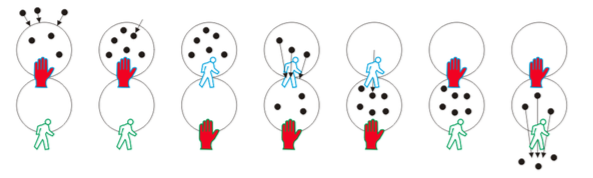
\includegraphics[width=\textwidth]{images/reusable-barrier.png}
\end{center}

This solution can also be called a \alert{two-phase barrier} because all threads have to wait twice: once at each turnstile.

\end{frame}

\begin{frame}[fragile]
\frametitle{Reusable Barrier Solution 3}
\vspace{-0.5em}
\textbf{Thread \textit{K}}\vspace{-0.5em}
  \begin{verbatim}
	 1. wait( mutex )
	 2. count++
	 3. if count == n
	 4.     wait( turnstile2 )
	 5.     post( turnstile1 )
	 6. end if
	 7. post( mutex )
	 8. wait( turnstile1 )
	 9. post( turnstile1 )
	10. [critical point]
	11. wait( mutex )
	12. count--
	13. if count == 0
	14.     wait( turnstile1 )
	15.     post( turnstile2 )
	16. end if
	17. post( mutex )
	18. wait( turnstile2 )
	19. post( turnstile2 )
  \end{verbatim}
\vspace{-2em}


\end{frame}


\end{document}

